\section{Illustrative Examples}

\subsection{Simulation of Models Having Different Component Types}
\begin{figure}
    \centering
    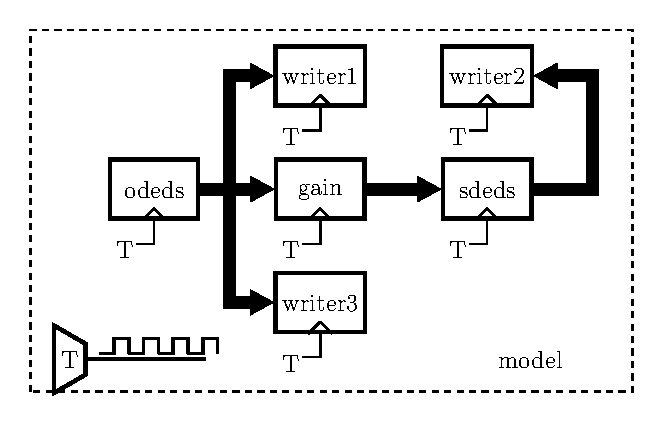
\includegraphics[width=\linewidth]{figures/CoupledChuaModel/coupled_chua_model.pdf}
    \caption{A model consisting of components represented by different equation types.}
    \label{fig: coupled model}
\end{figure}

In Causal.jl, it is possible to simulate models that include components represented by different types of equations. In Figure \ref{fig: coupled model} is given such an example model.`odeds` is a dynamical system represented by the ordinary differential equation in (\ref{eq: coupled ode}) where where $x_1, y_1, z_1$ are the state variables and $a=35, b=3, c = 28$ are system parameters.
\begin{equation}
    \begin{split}
        \dot{x}_1 &= a (y_1 - x_1) \\
        \dot{y}_1 &= (c - 1) x_1 + c y_1 - x_1 z_1 \\
        \dot{z}_1 &= x_1 y_1 - b z_1
    \end{split}
    \label{eq: coupled ode}
\end{equation}
`sdsds` is dynamical system that is represented by the stochastic differential equation in (\ref{eq: coupled sde}) where $x_2, y_2, z_2$ are the state variables, $u=[u_1,u_2, u_3]$ is the input, $\eta$ is noise strength, $W_t$ is the Wiener process corresponding to the noise and $a, b, c$ are the same as those in (\ref{eq: coupled ode}).
\begin{equation}
    \begin{split}
        dx_2 &= (a (y_1 - x_1) + u_1) dt + \eta dW_t \\
        dy_2 &= ((c - 1) x_1 + c y_1 - x_1 z_1)dt + \eta dW_t \\
        dz_2 &= (x_1 y_1 - b z_1 + u_3) dt + \eta dW_t 
    \end{split}
    \label{eq: coupled sde}
\end{equation}
`gain` is a static system whose input output relation is given in (\ref{eq: gain}) where $u, y, \epsilon$ are the input, output and gain coefficient of the system. 
\begin{equation}
    y = \epsilon u
    \label{eq: gain}
\end{equation}
`writer1` and `writer2` are used to record the outputs of `odeds` and `sdeds`, respectively, while `writer3` is used to record the fast Fourier transform(FFT) of the data flowing out of `odeds`\cite{proakis2004digital}. 

Being a domain-specific-language, Causal.jl provides a syntax for handy model construction. The program written using Causal.jl to construct and simulate the model in Figure \ref{fig: coupled model} is given in Listing \ref{lst: coupled codes}. The program first starts with the type definitions of the components `odeds`, `sdeds`, and `gain`, together with their fields' default values. Note that the types of components are defined as subtypes of the corresponding abstract component types, which shows how the user-defined component types can enrich the standard library of Causal.jl. `writer1` and `writer2` are used directly to record the data without further processing, so they do not need additional data processing plugins.
On the other hand, rather than directly recording the data, `writer3` is used to process the data online, so it needs an additional plugin. `FFTPlug` is defined for this purpose, and `writer3` is equipped with an instance. For the sake of this example, we used the `fft` function \cite{fftw}. The model is constructed and simulated for $100$ seconds with a step size of $0.001$ seconds. After the simulation, the data in `write1` and `writer2` are read back and plotted in Figure \ref{fig: coupled simulation results}. From Figure \ref{subfig: coupled simulation sde}, the presence of the noise is apparent in the trajectory of `sdeds`. 

The individual evolution of components makes it possible to simulate such models that include components represented by different equations. 

Causal.jl adopts a causal modeling approach in which the data flow through the connections is unidirectional. Components that write data to a connection drives other components that read data from the same connection. Thus, the topological structure of a model can be extracted by following the components that read data from the connections bound to the output ports of model components.

The order in which the connections are specified is arbitrary. One does not need to follow the true data flow directions through the connections. Therefore, complex topologies with many components can be defined concisely.

\begin{figure}
    \centering
    \subfloat[]{
        \begin{tikzpicture}
            \node[](plt){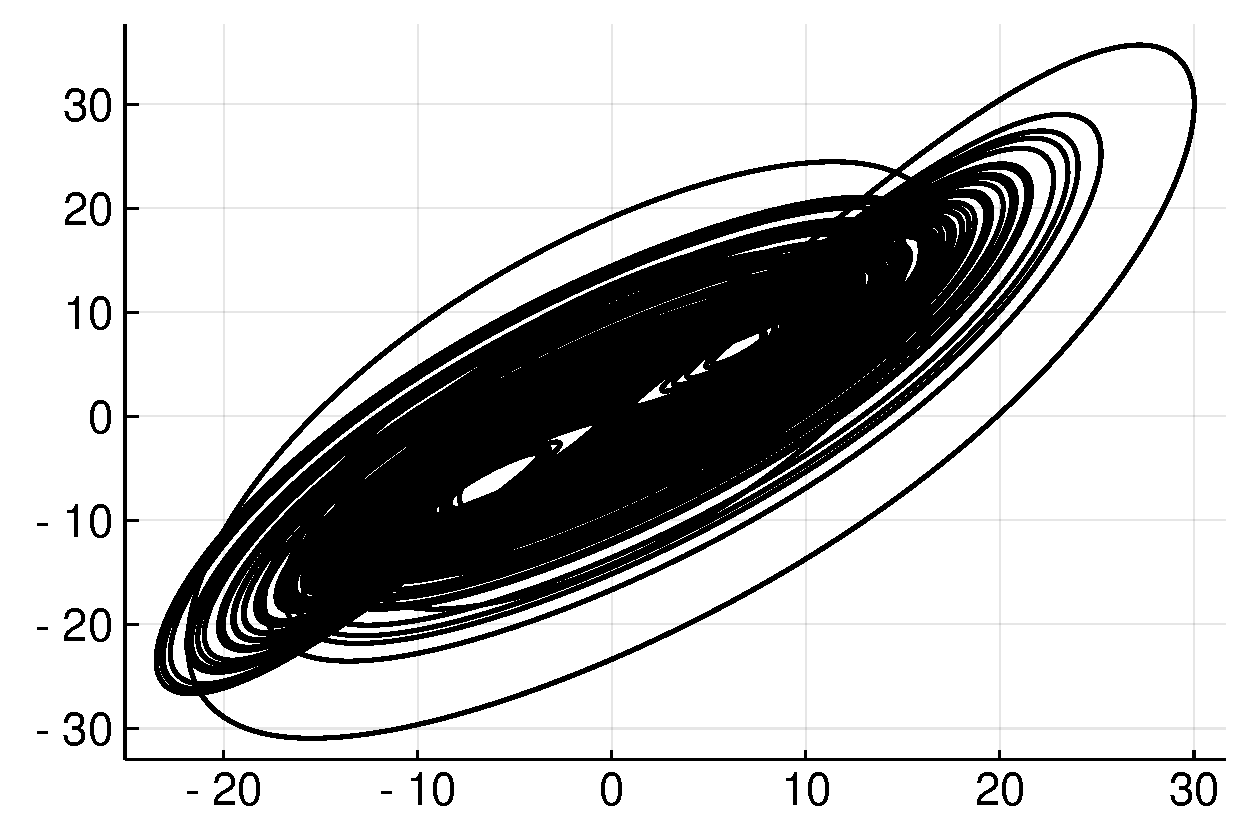
\includegraphics[scale=0.25]{figures/ChenSystemSimulations/odeds.pdf}};
            \node[] at (plt.south) {$x_1$};
            \node[] at (plt.west) {$y_1$};
        \end{tikzpicture}
        \label{subfig: coupled simulation ode}
        }\\
    \subfloat[]{
        \begin{tikzpicture}
            \node[](plt){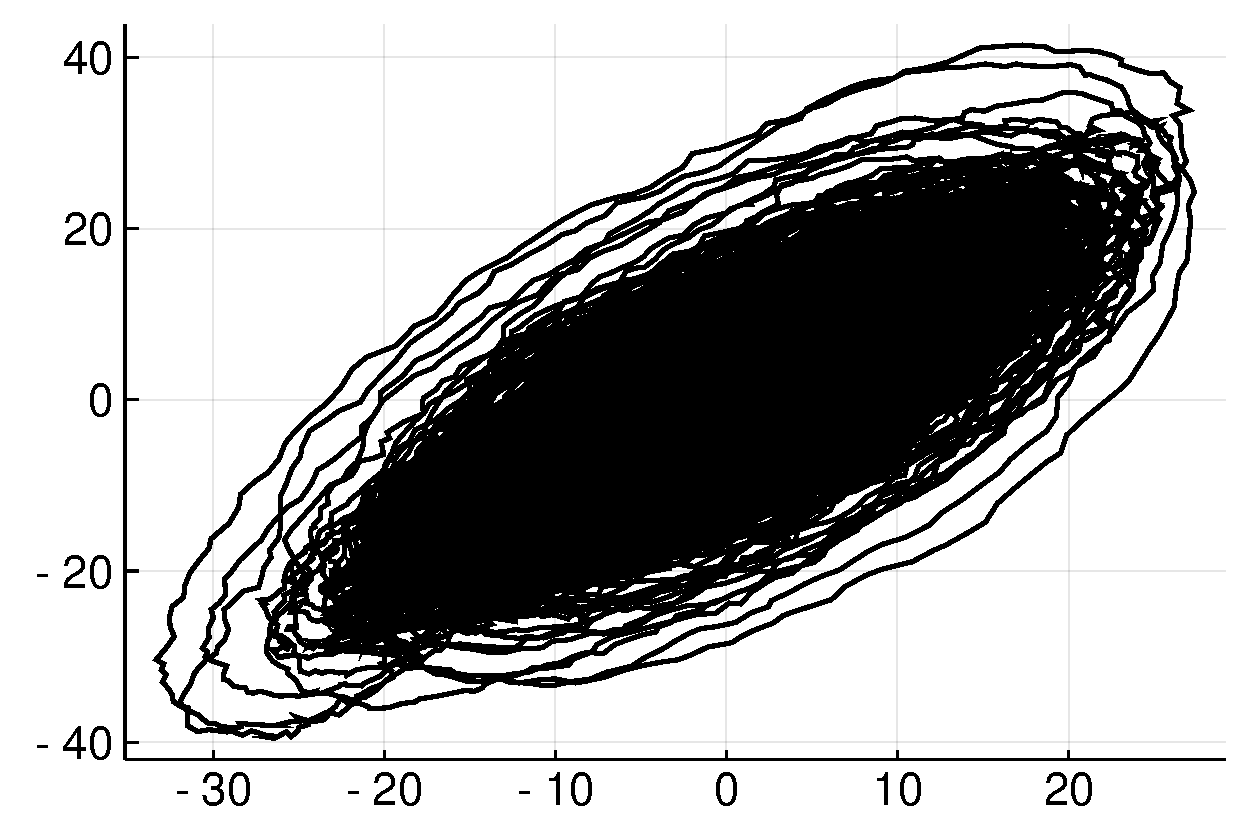
\includegraphics[scale=0.25]{figures/ChenSystemSimulations/sdeds.pdf}};
            \node[] at (plt.south) {$x_2$};
            \node[] at (plt.west) {$y_2$};
            \end{tikzpicture}
        \label{subfig: coupled simulation sde}
    }
    \caption{\protect\subref{subfig: coupled simulation ode} $x_1 - y_1$ trajectory of `odeds`. \protect\subref{subfig: coupled simulation sde} $x_2 - y_2$ trajectory of `sdeds`.}
    \label{fig: coupled simulation results}
\end{figure}


\subsection{Simulation of Models Consisting of a Large Number of Nodes}
In Causal.jl, its is possible to simulate large scale complex models consisting of a large number of dynamical system nodes. As an example, a network of continuous time identical dynamical systems is given Figure \ref{fig: network graph}. The nodes of the network evolve by 
\begin{equation}
    \dot{\bm{x}}_i = f(\bm{x}_i) + \bm{u}_i, \quad i = 1, \ldots, n
    \label{eq: network equation}
\end{equation}
where 
\begin{equation}
    \bm{u}_i = \sum_{i = 1}^n \epsilon_{ij} \bm{P} \bm{x}_j, \quad i = 1, \ldots, n,
    \label{eq: network node inputs}
\end{equation}
$n$ is the number of nodes, $\bm{x}_i \in \mathbb{R}^d$ is the state vector of node $i$, $f: \mathbb{R} \mapsto \mathbb{R}^d$ is the function corresponding to the individual node dynamics, $\epsilon_{ij} \geq 0 $ is the coupling strength between the nodes $i$ and $j$. The diagonal matrix $\bm{P} = diag(p_1, \ldots, p_d)$ determines by which state variables the nodes are connected to each other. The matrix $\bm{E} = [\epsilon_{ij}] \in \mathbb{R}^{n, n}, \; \epsilon_{ij} = \epsilon_{ji} \geq 0, \; \sum_{j = 1}^n \epsilon_{ij} = 0, i = 1, \ldots, n$ determines the network topology: if $\epsilon_{ij} > 0$, there is a connection between the nodes $i$ and $j$, if $\epsilon_{ij} = 0$, there is no connection between the nodes $i$ and $j$.

In the network given in Figure \ref{fig: network graph}, $n=50$,  $f$ is the Lorenz dynamics given by,
\begin{equation}
    \begin{split}
        \dot{x}_{i,1} &= \sigma (x_{i, 2} - x_{i, 1}) \\
        \dot{x}_{i,2} &= x_{i, 1} (\rho -  x_{i, 3}) - x_{i, 2} \\
        \dot{x}_{i,3} &= x_{i, 1} x_{i, 2} - \beta x_{i, 3}
    \end{split}
\end{equation}
where $\sigma=10, \beta=8/3, \rho=28$ are system parameters, $\bm{P} = diag(1, 0, 0)$. The network has Wattz-Strogatz topology that has a vertex degree of $10$ and that is randomized with a probability of $0.5$\cite{watts1998collective}.

\begin{figure}
    \centering
    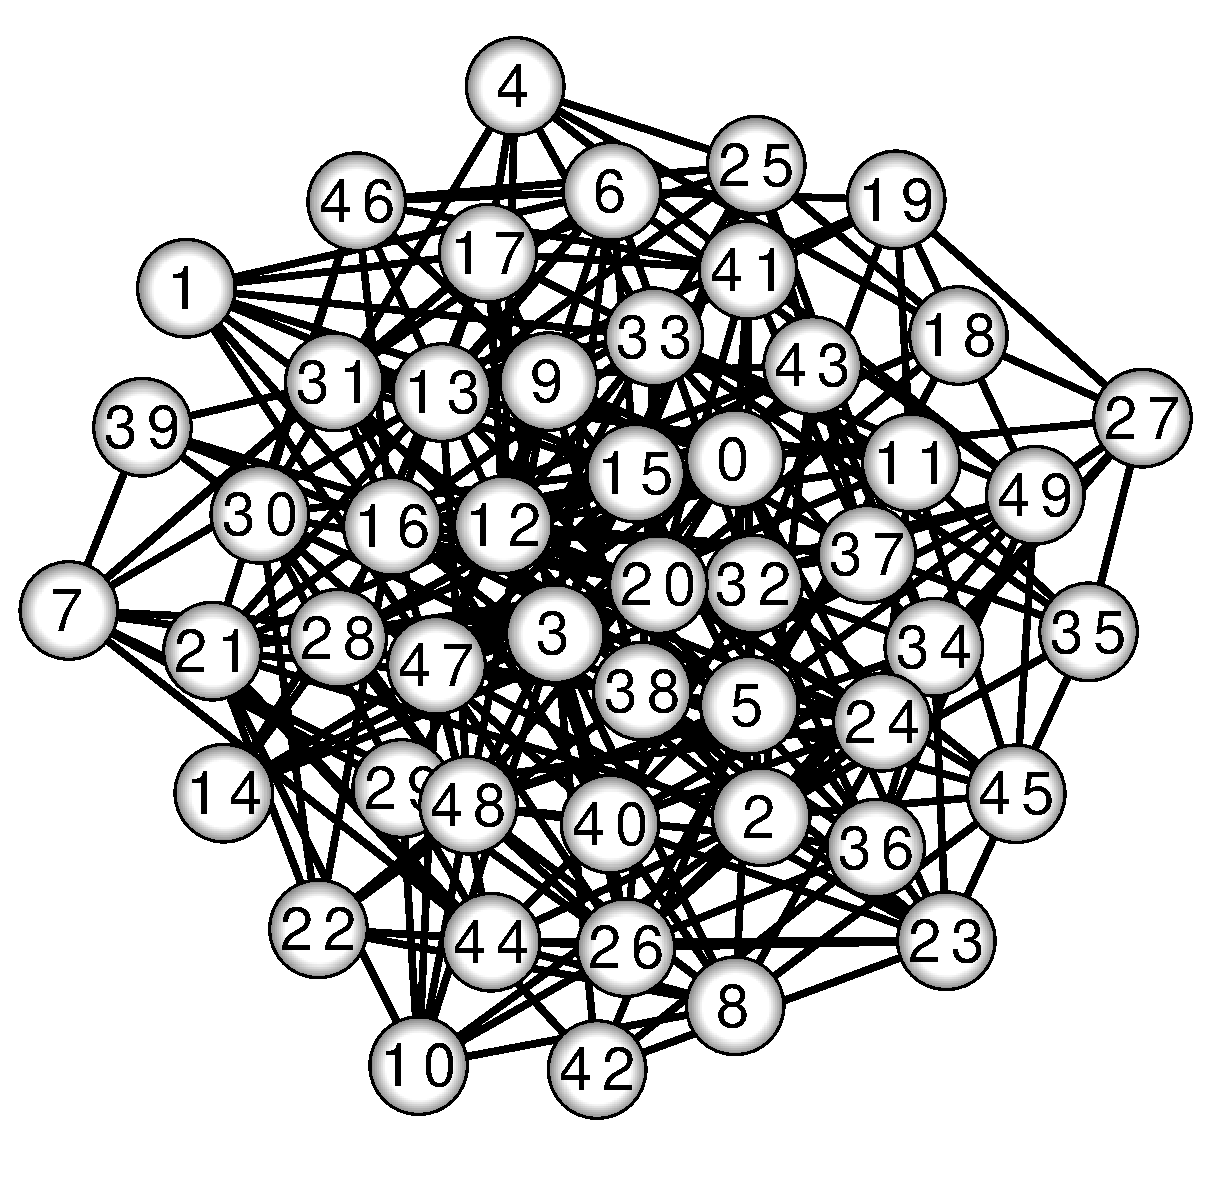
\includegraphics[width=0.5\linewidth]{figures/Networks/wattz_strogatz.pdf}    
    \caption{A network consisting of identical dynamical system nodes The spheres and the line segments represent the dynamical system nodes and the connection between them, respectively. s}
    \label{fig: network graph}
\end{figure}

The model in Figure \ref{fig: network graph} is given in Figure \ref{fig: network model}. `node $k$` for $k =1, \ldots, n$ correspond to the dynamical system nodes of the network.  From (\ref{eq: network equation}) and (\ref{eq: network node inputs}), we see that the states of the nodes are taken as their outputs, weighted by the coupling strengths and fed back to their inputs. Hence, `coupler` is used to construct the weighted outputs. `writer` records the nodes' outputs. The model has algebraic loops $L_k$ for $k = 1, \ldots, n$, where the algebraic loop $L_k$ consists of `node $k$` and `coupler`. 

\begin{figure}
    \centering
    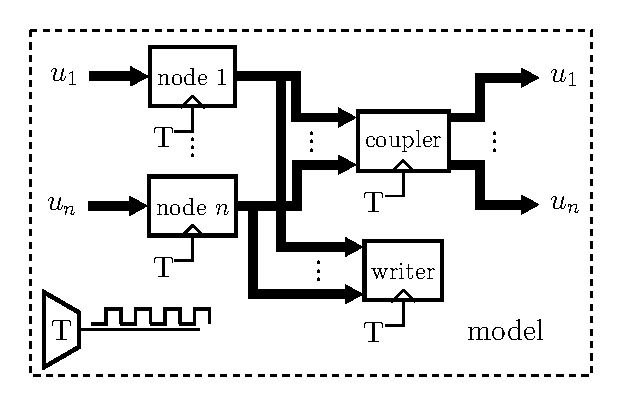
\includegraphics[width=0.8\linewidth]{figures/NetworkModel-WattzStrogatz/network_wattz_strogratz.pdf}
    \caption{Block diagram model of the network in Figure \ref{fig: network graph}.}
    \label{fig: network model}
\end{figure}

The program written using Causal.jl to construct and simulate the model in Figure \ref{fig: network model} is given in Listing \ref{lst: network codes}. Having defined the types of dynamical system nodes and the coupler, the model is constructed and simulated for $100$ seconds with a sampling period of $0.005$ seconds. After the simulation, the simulation data is read back from the writer and the mean square error (MSE) 
\begin{equation}
    MSE(t) = \dfrac{1}{n} \sum_{i = 2}^n \Vert \bm{x}_{1,1}(t) - \bm{x}_{i,1}(t) \Vert
\end{equation}
is computed and plotted. It is seen from Figure \ref{subfig: network error} that the all the nodes in the network synchronize with each other as the MSE goes to zero as time evolves. 

Note from the program in Listing \ref{lst: network codes} that memory components are not used to break algebraic loops of the model. Causal.jl is capable of detecting and breaking these algebraic loops automatically without requiring any user intervention. 

% TODO: Include package limits 1. Distributed simulation, breaking nested loops, subsystem construction.

\begin{figure}
    \centering
    \subfloat[]{
        \begin{tikzpicture}
            \node[](plt){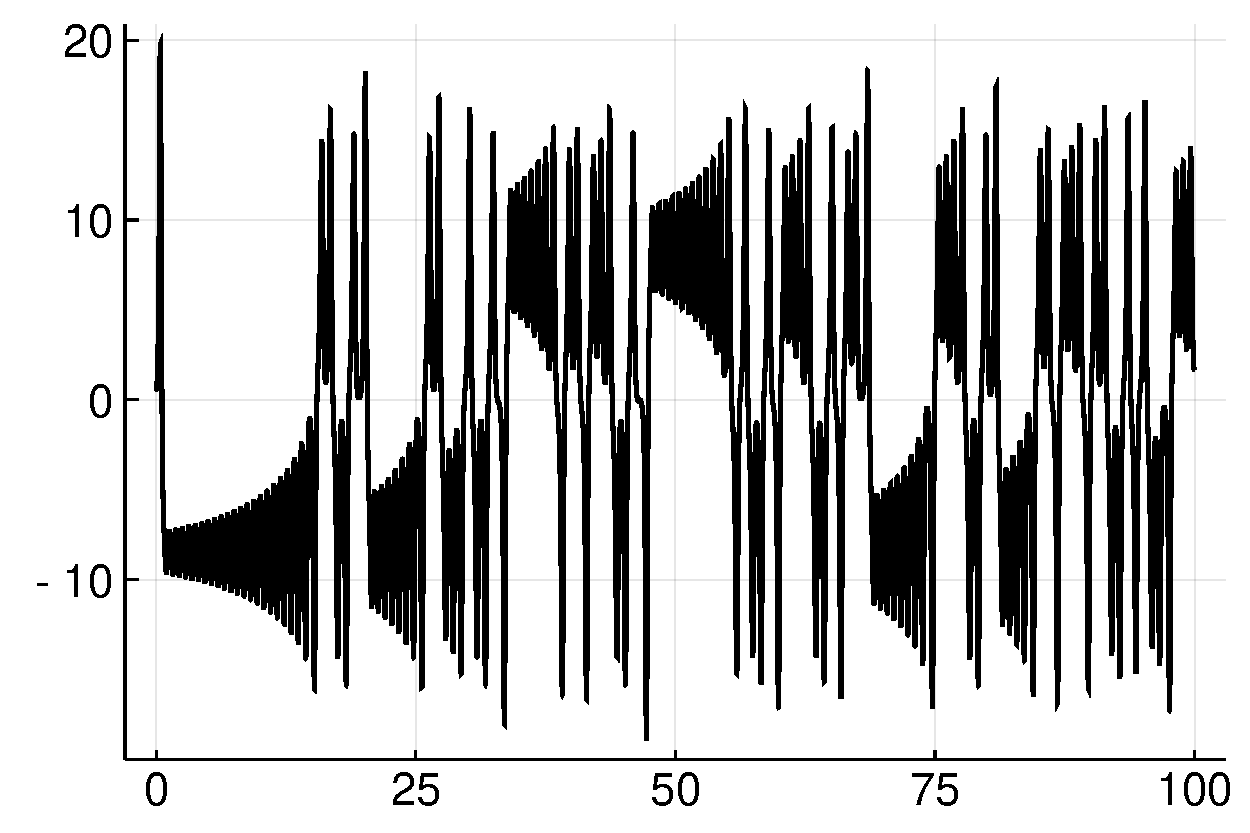
\includegraphics[scale=0.25]{figures/NetworkSimulation-WattzStrogatz/waveform.pdf}};
            \node[] at (plt.south) {$t$ [seconds]};
            \node[] at (plt.west) {$x_{1,1}$};
        \end{tikzpicture}
        \label{subfig: network timewaveform}
        }\\[-0.1cm]
    \subfloat[]{
        \begin{tikzpicture}
            \node[](plt){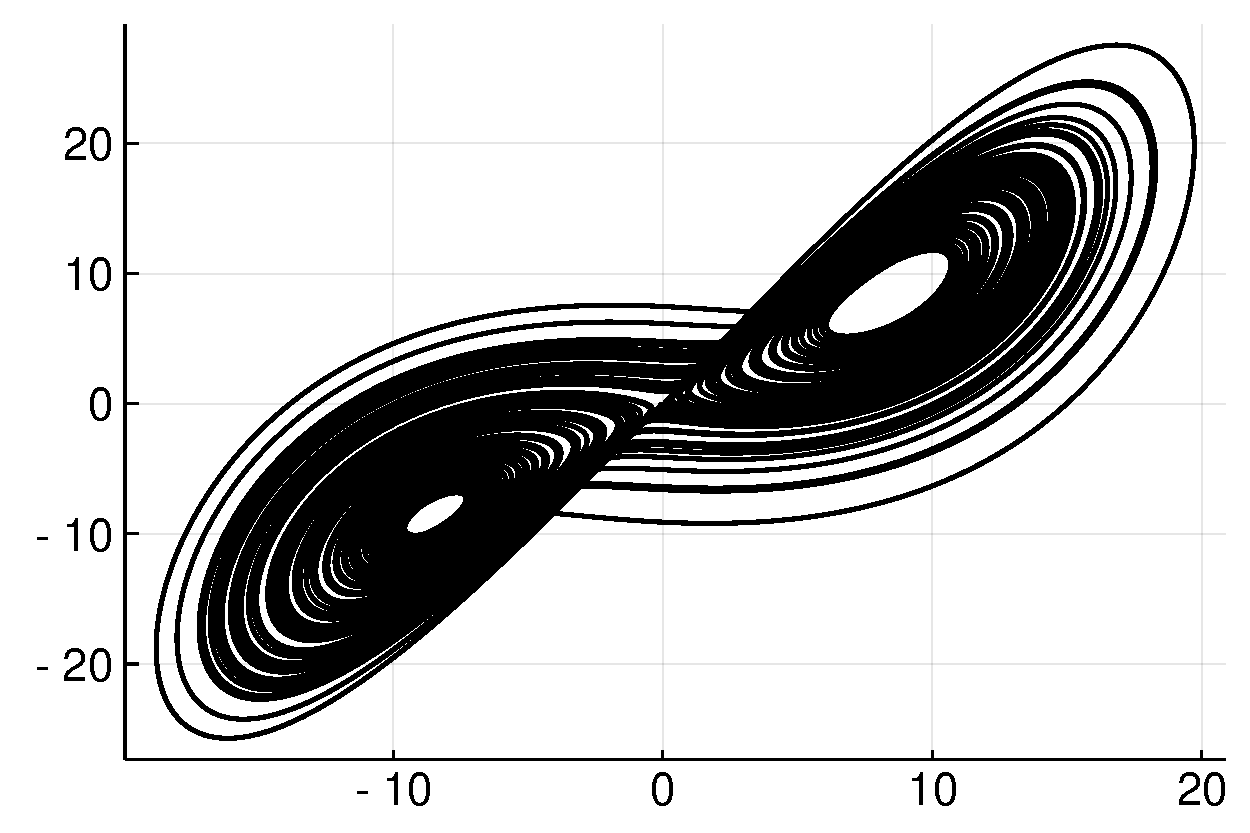
\includegraphics[scale=0.25]{figures/NetworkSimulation-WattzStrogatz/trajectory.pdf}};
            \node[] at (plt.south) {$x_{1,1}$};
            \node[] at (plt.west) {$x_{1, 2}$};
            \end{tikzpicture}
        \label{subfig: network trajectory}
    } \\[-0.1cm]
    \subfloat[]{
        \begin{tikzpicture}
            \node[](plt){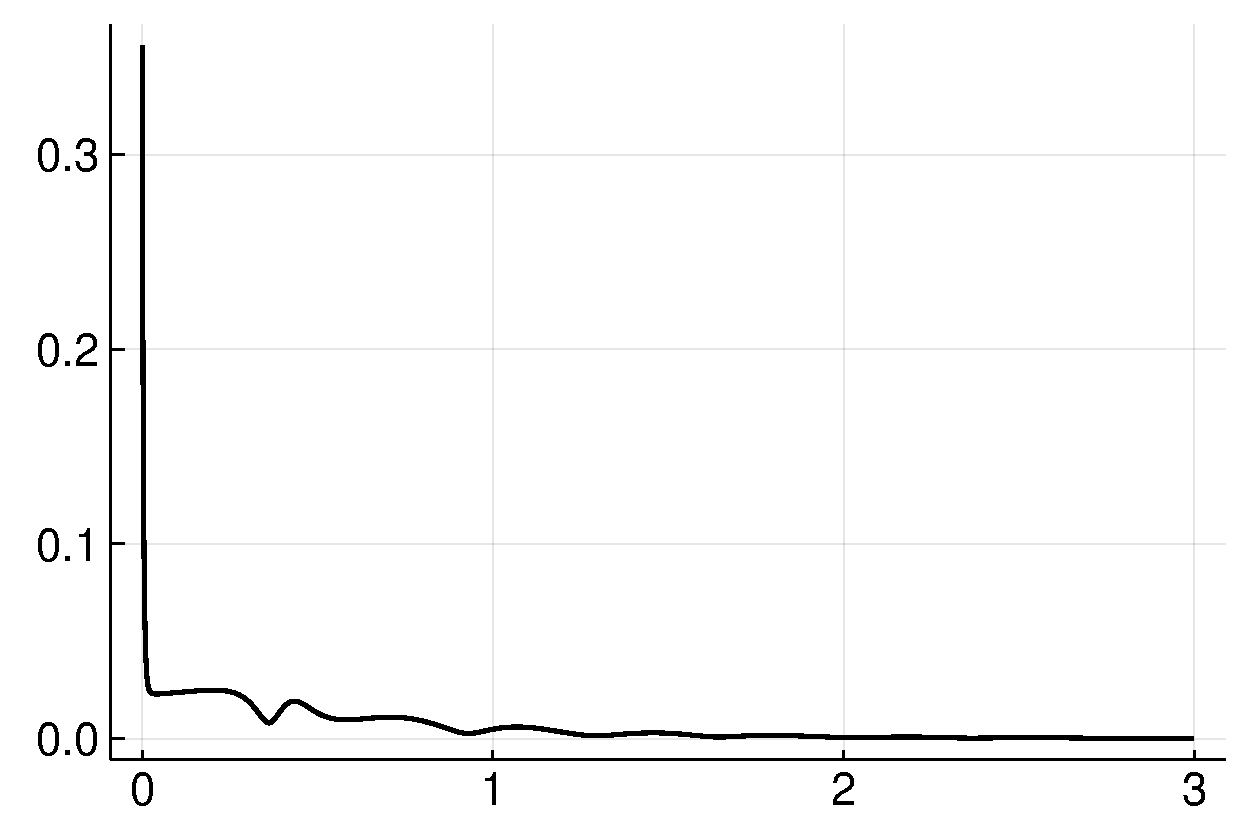
\includegraphics[scale=0.25]{figures/NetworkSimulation-WattzStrogatz/error.pdf}};
            \node[] at (plt.south) {$t$ [seconds]};
            \node[xshift=-0.25cm] at (plt.west) {MSE};
            \end{tikzpicture}
        \label{subfig: network error}
    }
    \caption{Simulation results the model given in Figure \ref{fig: network model}. \protect\subref{subfig: network timewaveform} Time waveform of $x_{1,1}$. \protect\subref{subfig: network trajectory} $x_{1,1} - x_{1,2}$ trajectory. \protect\subref{subfig: network trajectory} MSE.}
    \label{fig: network simulation results}
\end{figure}


% \subsection{Breaking Algebraic Loops}
% Consider the model given in Figure \ref{fig: small network}. The model includes dynamical systems `ds1` and `ds2` whose dynamics evolve by
% \begin{equation}
%     \begin{split}
%         \dot{x}_{i,1} &= \sigma (x_{i,2} - x_{i,1}) + u_i \\
%         \dot{x}_{i,2} &= x_{i,1} (\rho - x_{i,3}) - x_{i,2} \\
%         \dot{x}_{i,3} &= x_{i,1} x_{i,2} - \beta x_{i,3}
%     \end{split}
%     \qquad i = 1, 2.
%     \label{eq: small network noncompact}
% \end{equation}
% where $\sigma=10, \beta=8/3, \rho=28$ are the system parameters, $u_1 = \epsilon(x_{2,1} - x_{1,1})$, $u_2 = \epsilon(x_{1,1} - x_{2,1})$ and $\epsilon > 0$. (\ref{eq: small network noncompact}) can be written more compactly as
% \begin{equation}
%     \dot{\bm{x}} = \bm{f}(\bm{x}) + \epsilon(\bm{E}\otimes \bm{P})
% \end{equation}
% where $\bm{x} = [\bar{\bm{x}}_1, \bar{\bm{x}}_2], \; \bar{\bm{x}}_i = [x_{i, 1}, x_{i, 2}, x_{i, 3}], \; i = 1, 2$,
% \begin{equation}
%     \bm{E} = \begin{bmatrix*}[r]
%         -1 & 1 \\
%         1 & -1
%     \end{bmatrix*} \quad \bm{P} = \begin{bmatrix*}[r]
%         1 & 0 & 0 \\
%         0 & 0 & 0 \\
%         0 & 0 & 0 
%     \end{bmatrix*}, 
% \end{equation}
% and $\otimes$ is the Kronecker product. 

% \begin{figure}
%     \centering
%     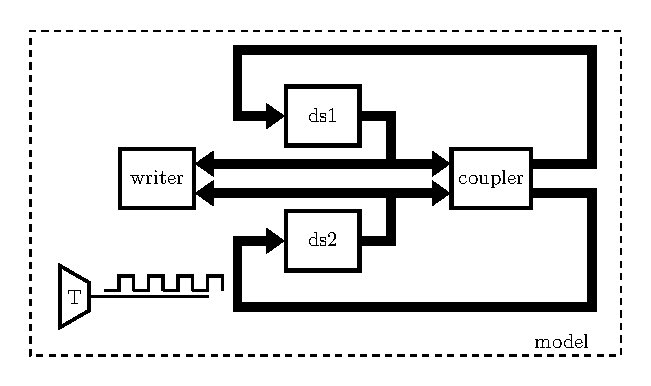
\includegraphics[width=\linewidth]{figures/SmallNetwork/small_network.pdf}
%     \caption{A model consisting algebraic loops.}
%     \label{fig: small network}
% \end{figure}

% Note from the block diagram of the model in Figure \ref{fig: small network} that there are feedback loops from the outputs of the dynamical systems to their inputs. This means there are algebraic loops in the model. The model includes two algebraic loops: the first loop is between `odeds1` and `coupler` and the second one is between `ds2` and `coupler`. It is possible to break these loops by inserting memory components in the loops. However, Causal.jl is capable of detecting and breaking algebraic loops automatically without requiring any user intervention. The program written using Causal.jl to construct and simulate the model in Figure \ref{fig: small network} is given in Listing \ref{lst: small network codes}. Having defined the component types, the model is constructed and simulated. After the simulation the data recorded into the writer component is read back and plotted in Figure \ref{fig: small network simulation results}. From the time waveform in Figure \ref{subfig: small network error}, as time evolves the absolute error between the $x_{1,1}$ state variable of `ds1` and $x_{2,1}$ goes to zero as time evolves, which implies two dynamical systems synchronize to each other.

% \begin{figure}
%     \centering
%     \subfloat[]{
%         \begin{tikzpicture}
%             \node[](plt){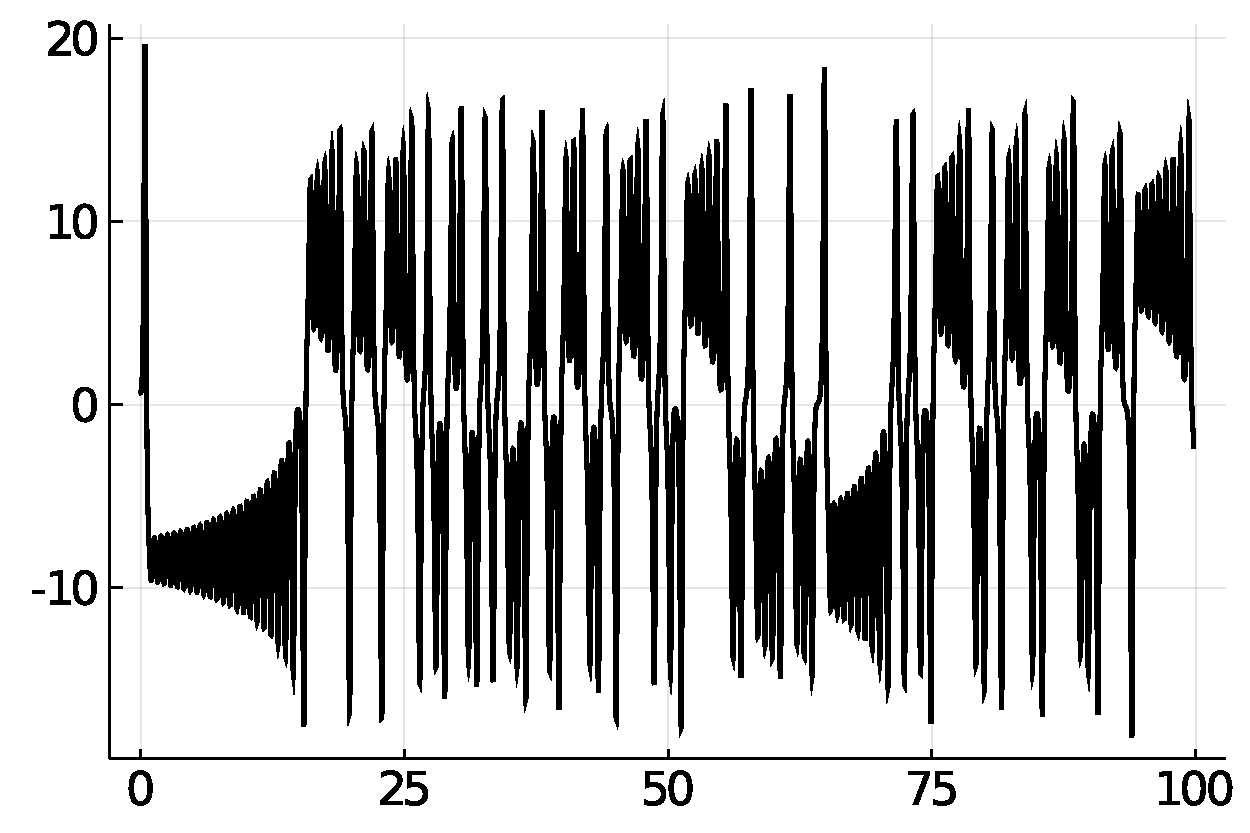
\includegraphics[scale=0.25]{figures/SmallNetworkSimulation/timewaveform.pdf}};
%             \node[] at (plt.south) {$t$ [seconds]};
%             \node[] at (plt.west) {$x_{1,1}$};
%         \end{tikzpicture}
%         \label{subfig: small network ds1}
%         }\\
%     \subfloat[]{
%         \begin{tikzpicture}
%             \node[](plt){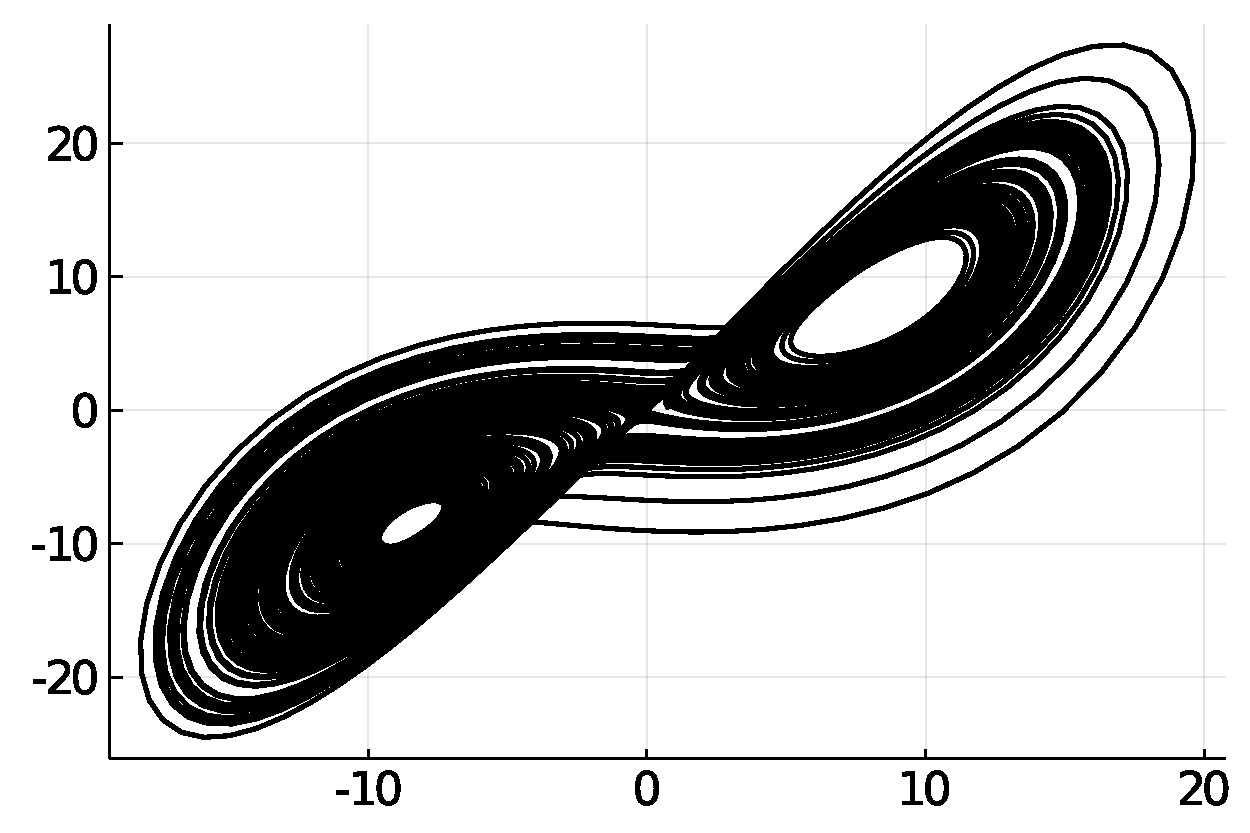
\includegraphics[scale=0.25]{figures/SmallNetworkSimulation/trajectory.pdf}};
%             \node[] at (plt.south) {$x_{1,1}$};
%             \node[] at (plt.west) {$x_{1,2}$};
%             \end{tikzpicture}
%         \label{subfig: small network ds2}
%     }\\
%     \subfloat[]{
%         \begin{tikzpicture}
%             \node[](plt){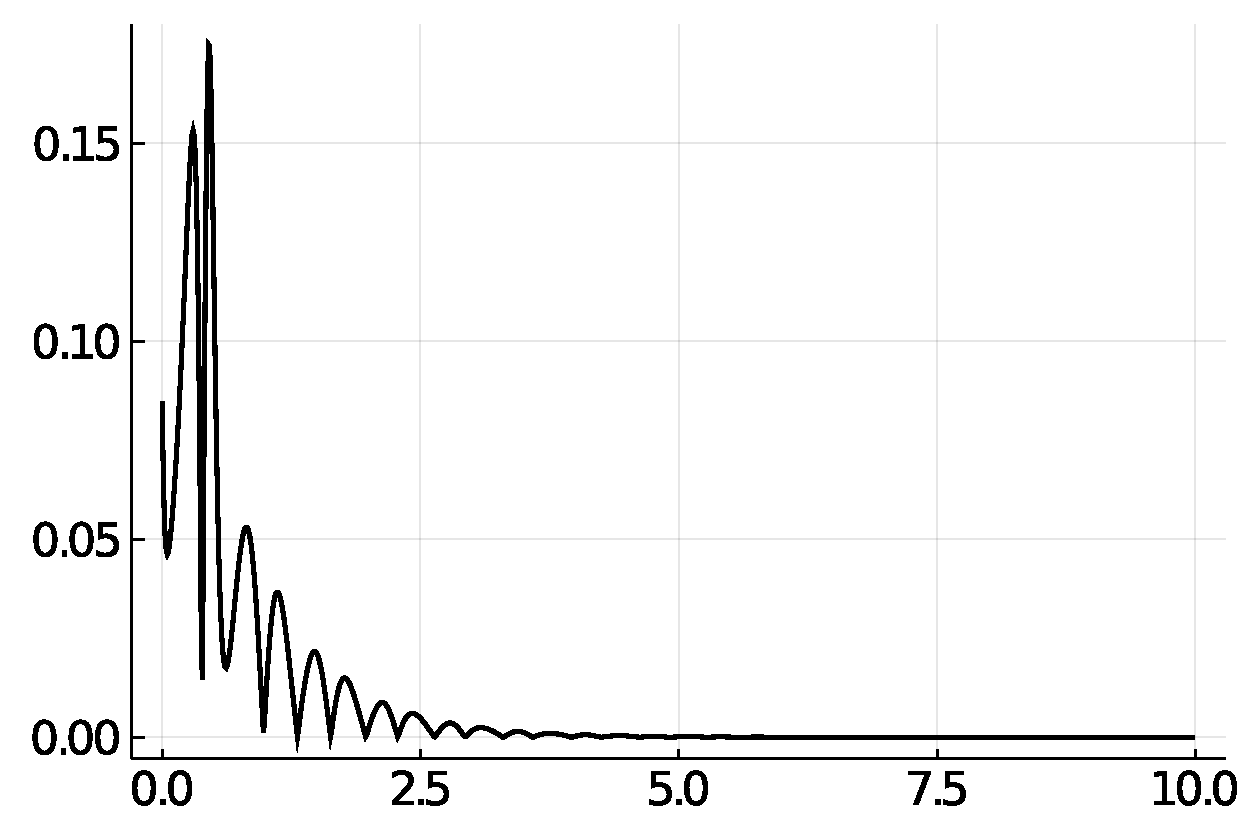
\includegraphics[scale=0.25]{figures/SmallNetworkSimulation/error.pdf}};
%             \node[] at (plt.south) {$t$ [seconds]};
%             \node[rotate=90] at (plt.west) {$|x_{1,1} - x_{2,1}|$};
%             \end{tikzpicture}
%         \label{subfig: small network error}
%     }
%     \caption{\protect\subref{subfig: small network ds1} Time waveform of $x_{1,1}$. \protect\subref{subfig: small network ds2} $x_{1,1} - x_{1,2}$ trajectory. \protect\subref{subfig: small network error}. The absolute error between $x_{1,1}$ and $x_{2,1}$}
%     \label{fig: small network simulation results}
% \end{figure}
